\documentclass[a4paper,10pt]{report}

\usepackage[utf8x]{inputenc}
\usepackage[francais]{babel}
\usepackage[T1]{fontenc}
\usepackage{graphicx}
\usepackage{fullpage}

\usepackage[colorlinks=true, urlcolor=blue, linkcolor=black]{hyperref}

\newcommand{\HRule}{\rule{\linewidth}{0.5mm}}

\begin{document}

  % Inclusion de la page de titre
  \begin{titlepage}

\begin{center}


\includegraphics[width=0.15\textwidth]{img/logo_ucbl.jpg}\\[1cm]

\textsc{\LARGE Moteur de Jeu de Stratégie Web}\\[1.5cm]

\textsc{\Large Projet TI5}\\[0.5cm]

% Title
\HRule \\[0.6cm]
{ \huge \bfseries Veille technologique}\\[0.4cm]

\HRule \\[1.5cm]

% Author and supervisor
\begin{minipage}{0.4\textwidth}
\begin{flushleft} \large
\emph{Auteurs:}\\
Ilyas \textsc{Boutebal}\\ Maxime \textsc{Colin}\\ Adrian \textsc{Gaudebert}\\ Youness \textsc{Hamri}\\ Van Duc \textsc{Nguyen}
\end{flushleft}
\end{minipage}
\begin{minipage}{0.4\textwidth}
\begin{flushright} \large
\emph{Client:} \\
Pierre-Antoine \textsc{Champin}
\end{flushright}
\end{minipage}

\vfill

% Bottom of the page
{\large \today}

\end{center}

\end{titlepage}
  
  % Sommaire
  \tableofcontents

  % Ajout d'une marge entre les paragraphes
  \setlength{\parskip}{0.1in}

\chapter{Compatibilité}
Le HTML5 et CSS3 sont des nouveautés à suivre ces temps-ci, et les navigateurs commencent à s’y adapter, mais à quel point ?

Voici quelques sites qui permettent de tester son navigateur, et de faire un petit bilan sur ce qui fonctionne, sur quel navigateur etc…

Html5 test.com : Ce site permet de réaliser un test de comptabilité d’un navigateur avec html5, et d’obtenir le résultat sous la forme d’un score sur 300.

caniuse.com: Dans ce site on trouve des tableaux récapitulatifs en fonction des différents standards et des navigateurs. Par contre, ce n’est pas très facile de s’y retrouver, mais le rappel des anciennes versions permet d’avoir une vue global de l’évolution.

FindMeByIP.com : C’est une application Web gratuite qui permet de déterminer quelles sont les caractéristiques valides des différents navigateurs, en particulier concernant : HTML5 et CSS3. L’outil analyse et fournit les informations concernant la compatibilité de chaque navigateur.

Pour conclure, quelques tableaux qui montrent la compatibilité de plusieurs navigateurs sur différents OS avec les différentes technologies.

\section{Propriétés CSS3}

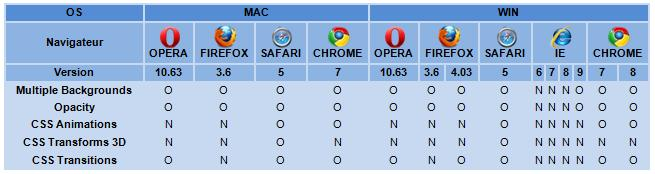
\includegraphics[width=420px]{img/CSS-Prop.jpg}

\section{Applications Web HTML5}

 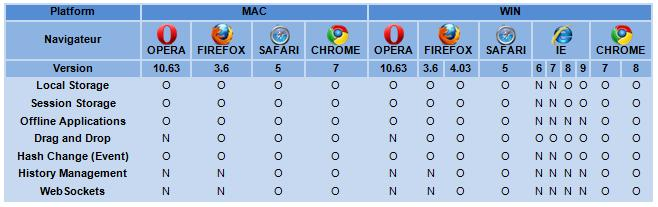
\includegraphics[width=420px]{img/HTML5-WebApp.jpg}

\section{Graphisme et contenu imbriqué HTML5}

 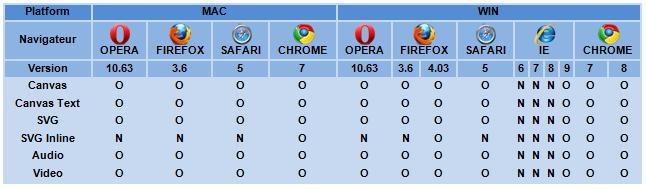
\includegraphics[width=420px]{img/Graphics.jpg}


Donc la question qui se pose est : faut-il utiliser ces nouvelles technos (HTML5, CSS3, canvas... ) dès aujourd'hui ?
Je pense que oui parce que :
\begin{itemize}
  \item Les balises HTML5 sont déjà en partie supportées par les navigateurs récents: Firefox, Safari, Chrome...
  \item Le HTML5 Canvas permet de créer des applications dynamiques / animées / de qualité équivalente à Flash... sans Flash!
  \item La lecture native de contenu media vidéo et audio dans la plupart des navigateurs.
  \item On peut utiliser « Chrome Frame » pour rendre compatible l'HTML5 sur les vieux navigateurs comme IE6, IE7.
  \item Les propriétés CSS3 sont déjà en partie supportées par plusieurs navigateurs récents comme Firefox, Safari, Chrome...
\end{itemize}

\chapter{Client}

\section{HTML5}
HTML5 est la dernière version de HTML, il introduit dans ses spécifications plusieurs 
balises, 
de nouveaux types et attributs pour les anciennes balises. 
On pourrait implémenter la majorité des fonctionnalités qu'on souhaite en HTML, couplé 
avec CSS et JavaScript, mais ce langage n'est pas conçus pour nos besoins, et on va donc 
chercher d'autres solutions plus adaptées. 

\section{Canvas}
Canvas est un composant de HTML5 qui permet d'effectuer des rendus dynamiques d'images 
bitmap via des scripts.
Canvas se résume donc en une zone de dessin dont la hauteur et la largeur sont définies 
dans du code HTML. Du code javascript permet d'accéder à l'aire via une série complète de fonctions de dessins, 
similaires aux autres API 2D, bien que permettant de générer dynamiquement des graphismes. Certaines personnes ont anticipé cet emploi de canvas en l'utilisant pour des graphiques, des animations et de la création d'images.
Le composant canvas est plutôt récent et n'est pour le moment implémentée que par 
quelques navigateurs: Firefox, Opéra, Safari, Konqueror, Google Chrome. 
Internet Explorer est encore en retard là-dessus mais l'arrivée de IE 9 permettra
 de le rattraper.

\begin{itemize}
  \item{Points forts}
  \begin{itemize}
    \item Dans un contexte hautement dynamique, la légèreté des images bitmap permet un traitement plus rapide des graphiques.
  \end{itemize}
  \item{Points faibles}
  \begin{itemize}
    \item La qualité des graphiques baisse en fonction de la taille de l'écran.
    \item Très jeune âge.
  \end{itemize}
\end{itemize}


 Sources:
\begin{itemize}
\item \url{http://fr.wikipedia.org/wiki/Canvas_(HTML)}
\item \url{https://developer.mozilla.org/fr/HTML/Canvas}
\end{itemize} 
	  

\section{SVG}
SVG est un format de données conçu pour décrire des ensembles de graphiques vectoriels. 
Il est basé sur XML. Les coordonnées, dimensions et structures de ces graphiques 
vectoriels sont indiqués sous forme numérique dans le document XML. 
Les couleurs et les polices de caractères à utiliser sont gérées par 
les feuilles de styles. 
En plus de la gestion de formes basiques (rectangles, ellipses, etc.), SVG gère
 des chemins (paths), qui utilisent les courbes de Bézier et qui permettent ainsi
 d'obtenir presque n'importe quelle forme.  D'autres outils lui permettent de gérer 
également le remplissage et la transparence des graphiques.

\begin{itemize}
\item Points forts
\begin{itemize}
\item Les graphiques vectoriels permettent de s'adapter aux différentes tailles d'écran, 
i.e. graphiques de très bonne qualité en toute circonstance.
\item Disponibilité de bibliothèques Javascript qui proposent des fonctionnalités de base 
et permettent de faciliter le travail des développeurs (i.e. raphael.js).
\item Il existe des logiciels graphiques qui permettent de modifier facilement chaque
 forme, par exemple en déplaçant des points, ou en changeant la couleur des traits, etc.
\end{itemize}
\item Points Faibles
\begin{itemize}
\item Le revers de la médaille de la qualité du graphisme est évidemment la consommation 
accrue de CPU (proportionnelle à la taille du graphique),
\item Rendement très faible dans un contexte très dynamique.
\item Ne permet pas de créer des points d'articulations, tels des noeuds dans un graphe. 
Bref, la notion de pointeur n'existe pas en SVG, ce qui rend la description de scènes 
dynamiques complexe.
\end{itemize} 
\end{itemize} 

Sources : \url{http://fr.wikipedia.org/wiki/Scalable_Vector_Graphics}

\section{Flash}
Les fichiers Flash, généralement appelés « animation Flash » portent l'extension .swf. 
Ils peuvent être inclus dans une page web et lus par le plugin Flash du navigateur, ou 
bien interprétés indépendamment dans le lecteur Flash Player. Flash est incontestablement 
une des méthodes les plus populaires pour ajouter des animations et des objets
 interactifs à une page web. 
Cependant, si Flash est une technologie très adaptée à nos besoins, elle est propriétaire
 et n'est donc pas compatible avec notre volonté de faire du « Web Ouvert ».
 
Sources : 

\begin{itemize}
  \item \url{http://pro.clubic.com/creation-de-site-web/langage-programmation/actualite-334796-cs5-flash-canvas-html5.html}
  \item \url{http://fr.wikipedia.org/wiki/Adobe_Flash#Flash_et_le_.C2.AB_Web_.C2.BB}
\end{itemize}

\section{Crafty.js}

Crafty.js est un framework JavaScript pour les jeux vidéos, dont le but est de fournir un ensemble de briques de bases et d'être très modulable. Il se base pour cela sur le modèle Composant / Entité\footnote{Cf. \url{http://cowboyprogramming.com/2007/01/05/evolve-your-heirachy} ou \url{http://www.gamearchitect.net/Articles/GameObjects1.html}} : chaque objet du jeu est une entité, et chaque entité est composée d'un ensemble de composants. Les différents composants de l'application contiennent les fonctionnalités du jeu. On aura par exemple une entité Unité qui aura pour composants ``2D, draw, health, clickable''. 

\subsection{Avantages}

\begin{itemize}
  \item Fourni un grand nombre de fonctionnalités nécessaires à notre moteur
  \item Architecture modulaire et extensible (possibilité d'ajouter, de manière simple, nos propres fonctionnalités)
  \item License libre (double license GPL et MIT)
\end{itemize}


\subsection{Inconvénients}

\begin{itemize}
 \item Pas de prise en charge native de SVG (uniquement canvas et DOM), mais possibilité d'étendre
 \item Framework très récent (actuellement en version 0.2) et maintenu par un seul développeur
\end{itemize}


\section{Comparatif}

  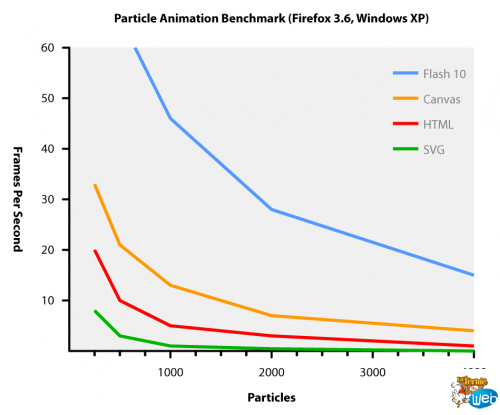
\includegraphics[width=420px]{img/bench.png}

  Le graphique ci-dessous nous donne un comparatif des quatre technologies dans 
un contexte très dynamique.
 
Le graphique ci-dessus donne un comparatif du rendement de ces quatre technologies sous 
Firefox (résultat similaire pour les autres navigateurs) et le résultat est sans appel: 
Flash l'emporte haut la main, canvas vient en deuxième position, HTML et SVG en dernière 
position. Le lien suivant donne un comparatif en image du rendement de ces technologies : \url{http://www.lafermeduweb.net/billet/un-bench-flash-vs-canvas-comparant-une-animation-de-particules-801.html}

\section{Conclusion}
Malgré la puissance de Flash, nous avons décidé de ne pas utiliser cette 
technologie pour rester dans l'esprit de l'open source.
Dans le contexte de notre moteur de jeux qui n'est pas très dynamique puisqu'au tour par tour, le large panel 
d'outils offert par SVG, grâce à son ancienneté et la qualité de ses graphiques,
 nous incite à choisir cette technologie. De plus, elle est largement supportée par les navigateurs
 (cf. Etude sur la compatibilité).



\chapter{Serveur}

  \section{TWISTED}
Twisted est un moteur réseau événementiel (event-driven networking engine) écrit en Python et sous licence MIT Free Software licence. Il contient un serveur Web, de nombreux client chat, de serveur chat, de serveur mail, et etc. Twisted supporte TCP, UDP, SSL/TLS, multicast, Unix domain sockets, un grand nombre de protocoles dont HTTP, NNTP, IMAP, SSH, IRC, FTP, et beaucoup d'autres.
\begin{itemize}
\item Le code source complet contient de nombreux Hooks pour le contenu dynamique.
\item Écrit en Python, un langage de haut niveau, Twisted offre la sécurité et la stabilité grâce à la classe la plus commune de réseau sécurité, le "buffer-overflow", et au mécanisme de Python pour gérer des erreurs. 
\item Servant les sites web à la haute circulation, le serveur web Twisted.web est configuré facilement.
\item Plusieurs APIs intégrés permettent aux développeurs de développer rapidement des nouveaux protocoles et des nouveaux services.
\item Simplement pour développer le client et serveur avec une même base de code (base-code).
\end{itemize}


\begin{figure}[!ht]
  \centering
  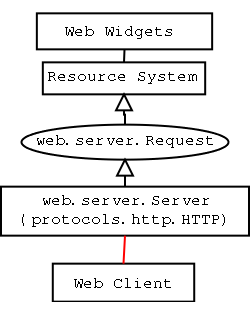
\includegraphics[scale=0.7, bb=0 0 251 314]{img/Twisted.png}     
\end{figure} 

Lorsque le Serveur reçoit une requête de Client, il crée un objet Request et l’envoie au système de ressources qui détermine l’objet Resource approprié à l’URL demandé par le Client.

  \section{TORNADO}
Tornado est la version open source de serveur web de FriendFeed racheté par Facebook. C’est un serveur d’application web asynchrone et non-blocking,  écrit en Python. Il peut traiter de nombreuses connections simultanée (les services Web en temps réel).


Tornado contient plusieurs modules : web, escape, database, template, httpclient, auth, locale, option,… Le module le plus important est le module web qui inclut la plupart des fonctionnalités principales de Tornado. Les autres modules sont les outils pour assister ce module.


Parmi les frameworks web Python, Tornade est le plus rapide.
\begin{figure}[!ht]
  \centering
  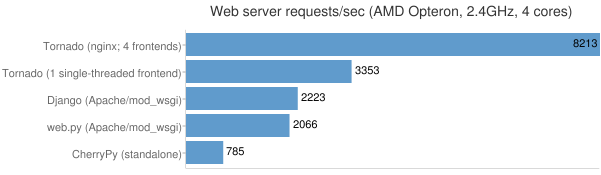
\includegraphics[scale=0.7, bb=0 0 601 175]{img/Tornado.png} 
\end{figure} 

  \section{COMET}
Ce sont les techniques permettant à un serveur web d'envoyer des informations au navigateur web sans que celui-ci l'ait explicitement demandé.  Il dépend des composants inclus par défaut dans les navigateurs web, tel que JavaScript. Cette approche diffère amplement du modèle classique du web où le navigateur demande un page web complet pour chaque fois.

Des méthodes spécifiques implémentant Comet tombe dans 2 major catégories:
\begin{itemize}
\item Streaming : Hidden IFrame, XMLHttpRequest
\item AJAX avec long polling : XMLHttpRequest long polling, Script tag long polling.
\end{itemize}

  \section{AJAX PUSH ENGINE PROJECT}
APE est une technologie permettant d'échanger des données entre des milliers d'utilisateurs via un navigateur web, sans recharger tout la page web.. APE n’utilise que les standards du web (avec AJAX), alors il est compatible avec tous les navigateurs web sur les ordinateurs et bien sur les appareils mobiles.


APE est devisé en 2 parties distinctes : La partie la plus centrale est le serveur APE  étant le serveur epoll-driven HTTP streaming. Et la partie APE JavaScript Framework envoie et reçoit les actions du côté client grâce aux les protocoles APE.

\begin{itemize}

 \item \textbf{Serveur APE:} étant un serveur COMET et écrit en C, le serveur APE implémente les méthodes POST et GEST du protocole HTTP. Il est utilisé uniquement pour AJAX Push.
  \begin{figure}[!ht]
    \centering
    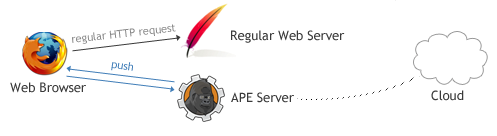
\includegraphics[scale=0.6, bb=0 0 497 136]{img/APEServeur.png} 
  \end{figure} 
 \item \textbf{APE JavaScript Framework:} reçoit des informations envoyées par le serveur (RAW), gère les données, et renvoie les commandes d’utilisateurs (CMD).
  \begin{figure}[!ht]
    \centering
    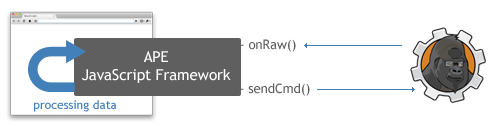
\includegraphics[scale=0.6, bb=0 0 500 127]{img/APEFramework.png} 
  \end{figure} 
\end{itemize}


L’advantage de l’APE le plus important est la vitesse du chargement. Il est entièrement adapté pour les connexions lentes telles que EDGE ou 3G.

  \section{RUBY EVENT MACHINE}
Eventmachine est une bibliothèque de programmation pour Ruby, C++, et Java. Il fournit event-driven I/O en utilisant le reactor pattern.  Le reactor pattern décrit un gestionnaire de service qui reçoit les événements et les envoie pour enregistrer. L’avantage du reactor pattern est la séparation entre répartition d’événements et l’application logique qui gère les événements, sans compliquer le code avec le multithreading.


Fondamentalement, eventmachine (EM) s'occupe de toutes ces choses au bas niveau: l'écoute sur les sockets, la création de connexions réseau, la gestion de TIMERS  et des simultanéités. 
  \begin{figure}[!ht]
    \centering
    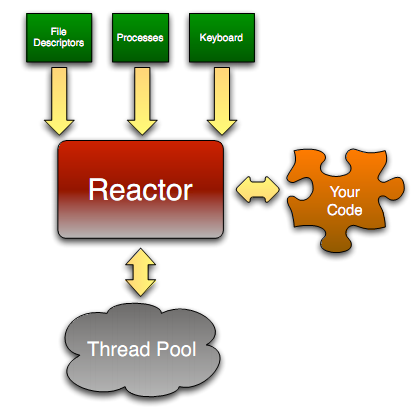
\includegraphics[scale=0.7, bb=0 0 414 415]{img/RubyEM.png} 
  \end{figure}


Eventmachine est conçu pour satisfaire simultanément 2 besoins principaux:
\begin{itemize}
 \item L’expansion, les performances et la stabilité
 \item Une API qui élimine la complexité de la haute performance de programmation réseau, permettant aux ingénieurs de se concentrer sur leur logique d'application.
\end{itemize}


L'idée de base: Au lieu d'attendre une réponse du réseau, EventMachine utilise ce temps pour traiter d'autres demandes. Il peut gérer 5000-10000 connexions simultanées avec un seul processus Ruby. 

  \section{NODE.JS}
Node.js est un framework Javascript qui s'exécute côté serveur, il est construit sur le moteur V8 (compilation à la volée), le très performant moteur JavaScript open source soutenu par Google et utilisé par le navigateur Chrome. Il permet de réaliser des applications web non-bloquantes, temps-réel (asynchrone), performantes, scalables.


Node.js utilise une boucle d'événements (event loop) au lieu de threads, et peut gérer des millions de connexions simultanées. Chaque opération I/O dans Node.js est asynchrone, ce qui signifie que le serveur peut continuer à traiter les demandes entrantes pendant que l’opération I/O se déroule.


Node.js fonctionne sur Linux, Mac OS X, FreeBSD. Windows ne supporte pas encore Node.js complètement.


Les avantages du langage JavaScript:
\begin{itemize}
 \item Le nombre de programmeur JavaScript est géant et il continue à augmenter.
 \item JavaScript est soutenu par presque tous les navigateurs (même sur les appareils mobiles).
 \item Il est en train de devenir l'une des langues les plus populaires.
\end{itemize}


Les avantages du Node.js:
\begin{itemize}
 \item JavaScript est fait pour l'évènementiel: la programmation par callback est familière aux développeurs d'applications AJAX et, pour se faire, la syntaxe des fonctions anonymes et le support des closures est adapté.
 \item Node est construit sur Javascript: de part sa présence dans les navigateurs, c'est peut-être le language le plus programmé au monde et bénéficie de 15 ans d'expérience.
 \item Node se stabilise: l'API de Node gagne en maturité et est proche de se finaliser.
 \item Node est simple et petit: la documentation se promène d'un seul regard et permet de rapidement connaitre ses fonctionnalités.
 \item Node est rapide: le moteur V8 et l'architecture non bloquante en font l'une des architectures les plus puissantes du marché, spécialement pour les requêtes longues et intensives en I/O. 
\end{itemize}

  \section{CONCLUSION}
En fait, tous ces technologies de serveur ont des avantages qui permettent de realiser des serveurs web non-bloquant, asynchrones, performants et scalables. 

En premier lieu, on sait qu'on ne voudra pas utiliser Ruby Event Machine, car il est écrit dans des langages dont nous n'avons pas les compétences. On préfèrera donc utiliser soit Python, soit JavaScript. 

APE Project pourrait être un choix judicieux si on choisi également de ne pas utiliser les WebSockets : il fournit une alternative élégante et fonctionnelle. 

Node.js a l'avantage d'utiliser le langage JavaScript, qui est également le langage côté client. L'utiliser permettrait donc de ne maitriser qu'un seul langage, et donc de gagner en efficacité sur le projet. De plus, il semble très bien adapté à nos besoins. 

Les serveurs Twisted et Tornado se distinguent peu au niveau des fonctionnalités dont nous avons besoin pour ce projet. 



  \paragraph{Sources}

    \begin{itemize}
    \item \url{http://twistedmatrix.com}
    \item \url{http://www.tornadoweb.org/documentation}
    \item \url{http://en.wikipedia.org/wiki/Comet_(programming)}
    \item \url{http://www.ape-project.org/ajax-push.html}
    \item \url{http://nodejs.org/}
    \end{itemize}




\chapter{Communication}

Cette partie concerne les technologies de communication client/serveur et 
client/client. Les différentes pistes retenu sont les WebSockets, Ajax, 
Opera Unite.

  \section{WebSocket}

    \subsection{Présentation}

WebSocket est une technologie fournissant un canal de communication bidirectionnel 
et fullduplex à travers un socket TCP. Il a été conçu pour être implémenté dans 
les navigateurs et serveurs web, mais il peut être utilisé dans n'importe quelle 
application client ou serveur. L'API WebSocket est en phase de standardisation 
par le W3C et le protocole par IETF.

Un tel canal de communication permet :

\begin{itemize}
  \item la notification au client d'une modification d'état du serveur
  \item l'envoi de données du serveur au client sans que celui ci n'ait à faire de requête.
\end{itemize}

    \subsection{Implémentation et support coté client}

Le protocoles WebSocket est implémenté dans les navigateurs Chrome 4, Safari 5, 
Firefox 4 et Opera 11. Son support est néanmoins désactivé dans Firefox 4 et 
Opera 11 pour des raisons de sécurité. Il est possible de l'activer via dans les 
paramètres des deux navigateurs. Internet Explorer ne supporte pas WebSocket.


    \subsection{Implémentation et support coté serveur}

Le protocole nécessite également d'être implémenté côté serveur pour être 
utilisé. Il existe plusieurs implémentations côté serveur de WebSocket, 
dans différents langages (Java, Python, PHP, Javascript...) et sous 
différentes formes (extension apache, serveur entier, script...).

Quelques implémentations :

\begin{itemize}
  \item GNU WebSocket4J, une implémentation du protocole WebSocket en Java. 
  \item pywebsocket3, une implémentation en Python sous la forme d'une extension pour le serveur Apache.
  \item jWebSocket, implémentation Java côté serveur et JavaScript/HTML5 côté client.
  \item Implémentation de WebSocket avec node.js
\end{itemize}

    \subsection{Sécurité}

WebSocket comporte à l'heure actuel une faille de sécurité dans la phase 
de ``handshacke'' permettant de remplacer un fichier javascript par un malware. 
La faille se situe au niveau de l'API elle-même. C'est pourquoi son support 
est désactivé par défaut sous Firefox 4 et Opera 11 jusqu'à ce que la faille 
soit fixée.


  \section{Ajax}

    \subsection{Présentation}

Ajax (Asynchronous Javascript and XML) est un rassemblement de differents outils 
et méthodes de conception permettant de construire des application web dynamiques
basées sur différentes technologies web côté client.

Ajax est une combinaison de technologies telles que JavaScript, XML, DOM et 
XMLHttpRequest dans le but de réaliser des applications Web qui offrent une 
maniabilité et un confort d'utilisation supérieur à ce qui se faisait jusqu'alors.

DOM et JavaScript sont utilisés pour modifier l'information présentée dans le navigateur 
par programmation. L'objet XMLHttpRequest est utilisé pour dialoguer de manière 
asynchrone avec le serveur Web. La notation XML est utilisée pour structurer les 
informations transmises entre le serveur Web et le navigateur.

En alternative au format XML, les applications Ajax peuvent utiliser les fichiers texte ou JSON.

  \subsection{Support}

Les applications Ajax fonctionnent sur tous les navigateurs Web qui mettent en oeuvre les 
technologies décrites précédemment, parmi lesquels Mozilla Firefox, Internet Explorer, 
Konqueror, Google Chrome, Safari et Opera.


  \section{Opera Unite}

    \subsection{Présentation}

Opera Unite est une technologie qui transforme un navigateur en serveur 
Web personnel. Avec Opera Unite, on devient à la fois client et serveur, 
à la fois visiteur et hôte. On reçoit du contenu du Web, et on en fournit 
également. On garde le contrôle : les données restent sur votre ordinateur, 
et on décide avec qui on désire les partager. 

    \subsection{Implémentations}

Opera Unite est implémenté dans le navigateur Opera depuis la version 10.


    \subsection{Conclusion sur Opera Unite}

Opera Unite est au final un service de partage de contenu et non de 
communication client/serveur, cette solution est donc inadaptée à nos 
besoins. De plus, cette fonctionnalité n'est disponible que sur le 
navigateur Opera.

  \section{Conclusion}

En conclusion, la technologie WebSocket semble la plus intéressante pour notre projet.
Elle semble adaptée à nos besoins. Néanmoins le fait que le protocole soit 
encore en phase de développement et le fait qu'il soit désactivé par défaut 
sur certains navigateurs pourrait poser problème.

Ajax semble également correspondre à certaines de nos attentes, mais dispose de plus
de restrictions au niveau communication client/serveur.


\chapter{Formats de données}

  \section{JSON}

    \subsection{Présentation}

JSON (JavaScript Object Notation) est un format de données textuel, 
générique, dérivé de la notation des objets du langage ECMAScript. 
Il permet de représenter de l’information structurée. Créé par Douglas 
Crockford, il est décrit par la RFC 4627 de l’IETF.


Un document JSON ne comprend que deux éléments structurels : 
\begin{itemize}
 \item des ensembles de paires nom / valeur ; 
 \item des listes ordonnées de valeurs. 
\end{itemize}


Ces mêmes éléments représentent 3 types de données : 
\begin{itemize}
  \item des objets ; 
  \item des tableaux ; 
  \item des valeurs génériques de type tableau, objet, booléen, nombre, chaîne ou null. 
\end{itemize}

Le format JSON est très facilement exploitable et manipulable en Javascript. 
Un document JSON représente un objet. Il est donc potentiellement plus facile 
à manipuler qu'un document XML.

    \subsection{Exemple}

\begin{verbatim}
{"menu": {
   "id": "file",
   "value": "File",
   "popup": {
     "menuitem": [
       {"value": "New", "onclick": "CreateNewDoc()"},
       {"value": "Open", "onclick": "OpenDoc()"},
       {"value": "Close", "onclick": "CloseDoc()"}
     ]
   }
 }}
\end{verbatim}

    \subsection{Sources}

\begin{itemize}
 \item \url{http://fr.wikipedia.org/wiki/Json}
\end{itemize}


  \section{XML}

    \subsection{Présentation}

Extensible Markup Language est un langage informatique de balisage générique. 
Il sert essentiellement à stocker/transférer des données de type texte Unicode 
structurées en champs arborescents. Ce langage est qualifié d’extensible car 
il permet à l'utilisateur de définir les balises des éléments. L'utilisateur 
peut multiplier les espaces de nommage des balises et emprunter les définitions 
d'autres utilisateurs

    \subsection{Exemple}

\begin{verbatim}
<menu id="file" value="File">
  <popup>
    <menuitem value="New" onclick="CreateNewDoc()" />
    <menuitem value="Open" onclick="OpenDoc()" />
    <menuitem value="Close" onclick="CloseDoc()" />
  </popup>
</menu>
\end{verbatim} 

    \subsection{Sources}

\begin{itemize}
 \item \url{http://fr.wikipedia.org/wiki/Xml}
\end{itemize}


  \section{HTML}

    \subsection{Présentation}

L’Hypertext Markup Language, généralement abrégé HTML, est le format de données 
conçu pour représenter les pages web. C’est un langage de balisage qui permet 
d’écrire de l’hypertexte, d’où son nom. HTML permet également de structurer 
sémantiquement et de mettre en forme le contenu des pages, d’inclure des 
ressources multimédias dont des images, des formulaires de saisie, et des 
éléments programmables tels que des applets. Il permet de créer des documents 
interopérables avec des équipements très variés de manière conforme aux exigences 
de l’accessibilité du web.

    \subsection{Sources}

\begin{itemize}
 \item \url{http://fr.wikipedia.org/wiki/Json}
\end{itemize}

  \section{Conclusion}

JSON et XML sont les deux format qui semblent les plus adaptés à nos besoin. 
JSON à un avantage au niveau de son interprétation par Javascript, une 
technologie certainement clé dans ce projet.

\end{document}
